\begin{figure}[h!]
    \begin{center}
    \caption{Effects on Public Health Spending per capita - By Type}\label{fig:7}
    \begin{subfigure}{0.48\textwidth}
        \centering
        \caption{\scriptsize Human Resources}\label{fig:7a}
        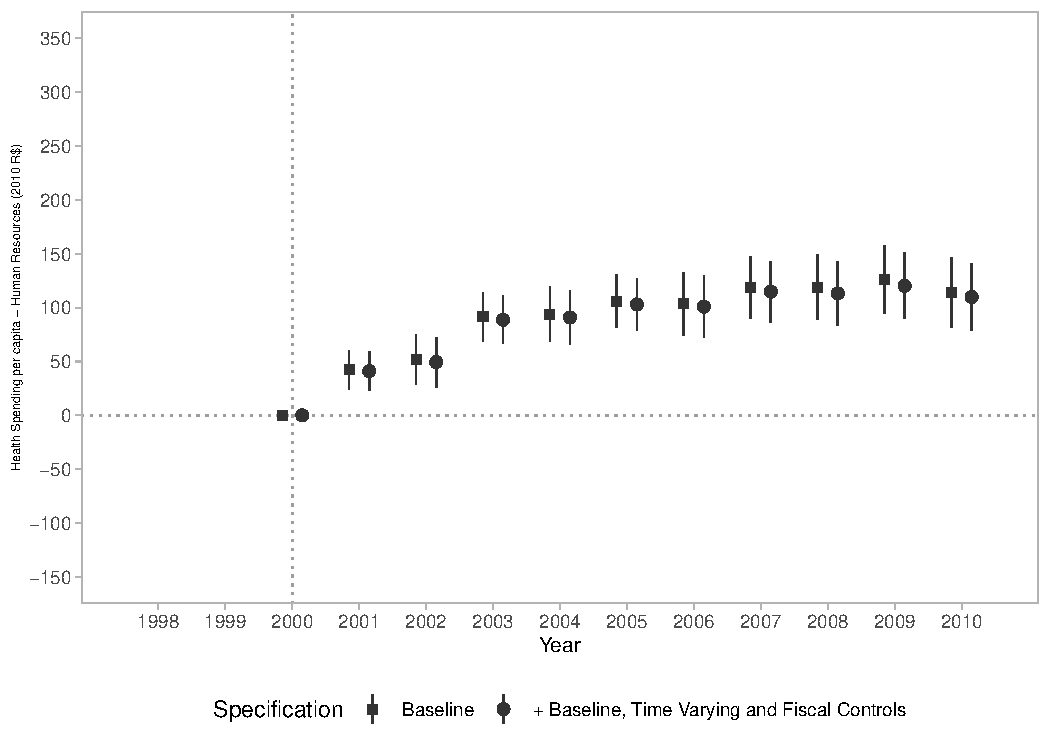
\includegraphics[width=\textwidth]{plots/siops_desppessoal_pcapita_dist_ec29_baseline_dist_ec29_baseline_7.pdf}
    \end{subfigure}
    \begin{subfigure}{0.48\textwidth}
        \centering
        \caption{\scriptsize Investment}\label{fig:7b}
        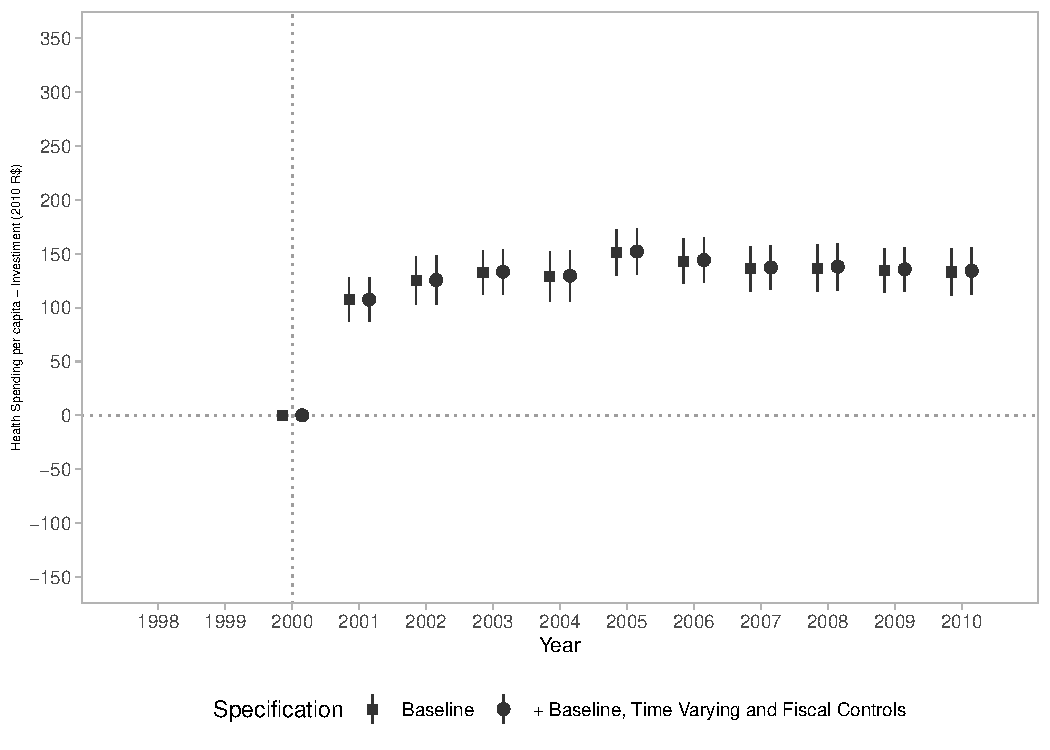
\includegraphics[width=\textwidth]{plots/siops_despinvest_pcapita_dist_ec29_baseline_dist_ec29_baseline_7.pdf}
    \end{subfigure}
    \begin{subfigure}{0.48\textwidth}
        \centering
        \caption{\scriptsize 3rd parties services}\label{fig:7c}
        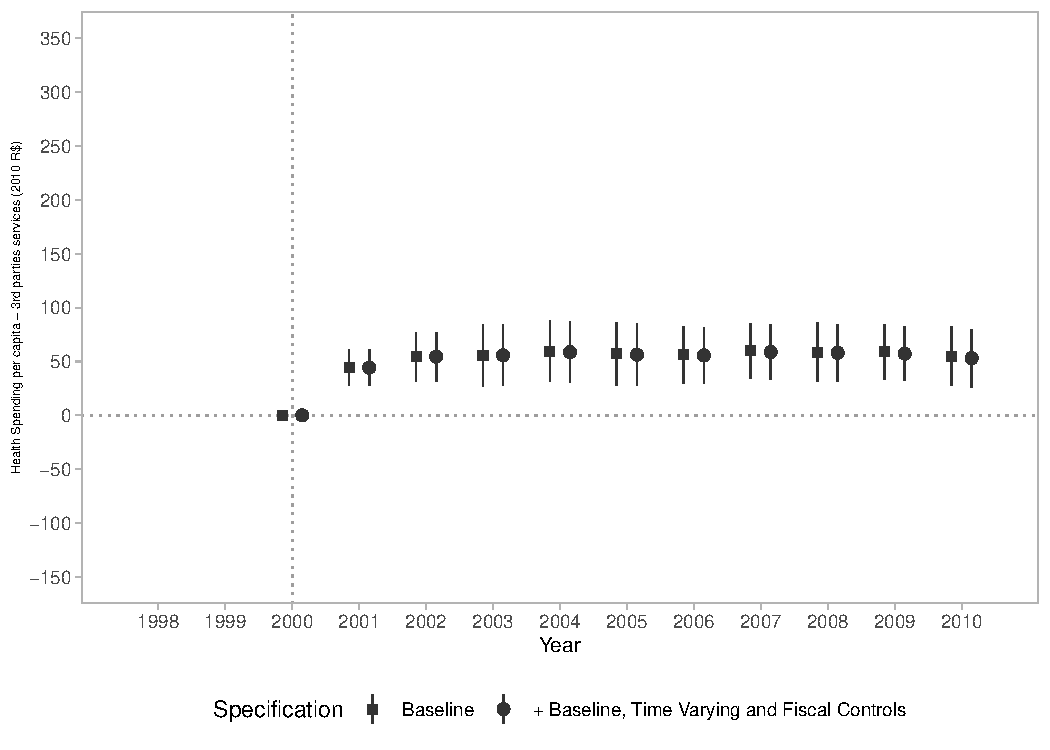
\includegraphics[width=\textwidth]{plots/siops_despservicoster_pcapita_dist_ec29_baseline_dist_ec29_baseline_7.pdf}
    \end{subfigure}
    \begin{subfigure}{0.48\textwidth}
        \centering
        \caption{\scriptsize Other Expenditures}\label{fig:7d}
        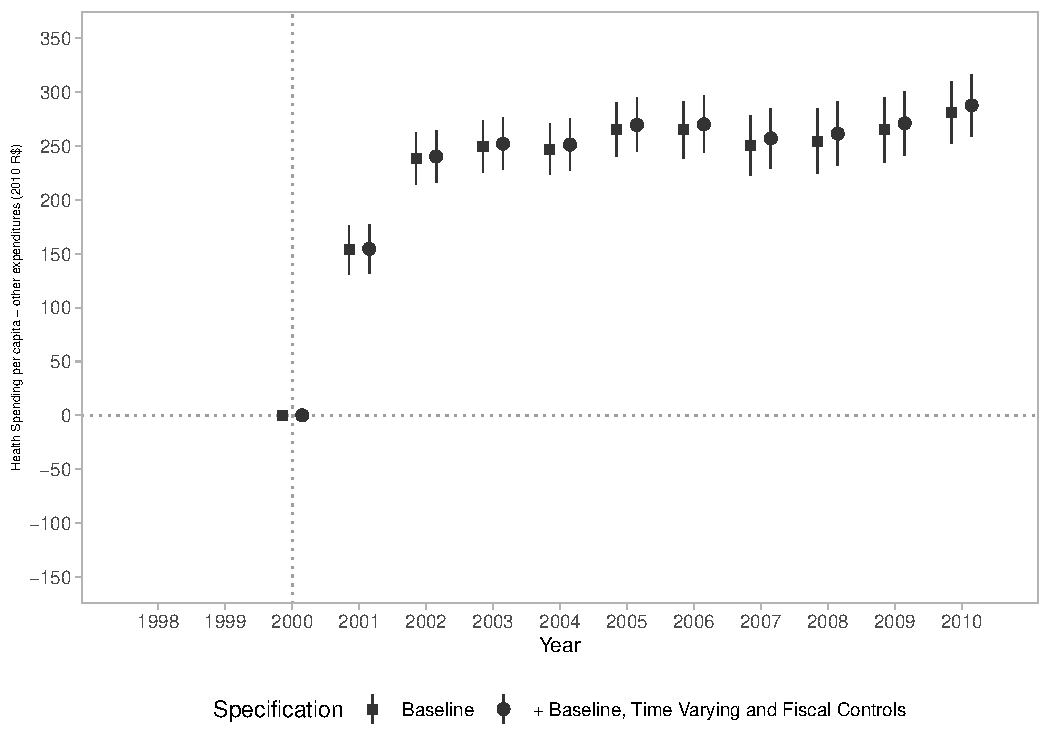
\includegraphics[width=\textwidth]{plots/siops_despoutros_pcapita_dist_ec29_baseline_dist_ec29_baseline_7.pdf}
    \end{subfigure}
    
    \end{center}
    
        \scriptsize{Notes: The number of observations is 55810. DiD Estimates from Equation \ref{eq:2}. Independent variable is the distance to the EC/29 target in p.p. Square dots represent the baseline model with municipality and state-year fixed effects. Round dots represent fully saturated specification (Column 4 in regression Tables). Lines represent 95\% confidence intervals. Arrows, when present, indicate confidence intervals out of the plot bounds. Standard errors are clustered in the municipality level.}
    
\end{figure}